\section{VM Volume storage}

\begin{frame}[t]{Intro}

	\note[item]{Σε μεγάλες εγκαταστάσεις, ξεφεύγουμε από το κλασσικό 
		μοντέλο του PC μας (το μηχάνημα έχει το σκληρό του δίσκο).  
		Συγκεκριμένα σε μια cloud υποδομή έχουμε:}
	\note[item]{\click}
	\note[item]{To VM που τρέχει σε ένα host server}
	\note[item]{\click}
	\note[item]{Και τους storage servers}
	\note[item]{\click}
	\note[item]{Το ερώτημα είναι λοιπόν, πως το VM θα αποθηκεύει τα 
		δεδομένα του;\\
		Υπάρχουν διάφορες επιλογές όπως το DRBD, το RBD που 
		χρησιμοποιούνται ευρέως και γεφυρώνουν τον αποθηκευτικό χώρο 
		του VM με το χώρο όπου λειτουργεί.}
	\note[item]{Τι γίνεται όμως στην περίπτωση που θέλουμε *και* τα εξής;}
	\note[item]{\click}
	\note[item]{Εξήγησε τους όρους}

	\begin{columns}[t]
		\begin{column}{.5\textwidth}
			\pause
			\makebox[\textwidth]{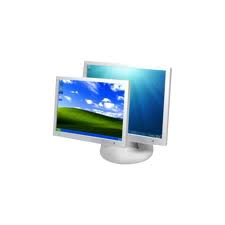
\includegraphics[width=.2\paperwidth]{images/vm.jpg}}
			\pause \centering{ {\Huge +} }
				\makebox[\textwidth]{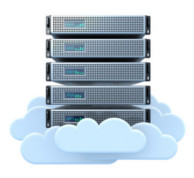
\includegraphics[width=.2\paperwidth]{images/cloud-server1.jpg}}
			\pause \centering{ {\Huge = ?}}
		\end{column}
		\begin{column}{.5\textwidth}
			\pause
			\begin{itemize}
				\item Policy enforcement?
				\item Storage agnosticity?
			\end{itemize}
		\end{column}
	\end{columns}

\end{frame}

\begin{frame}{Our solution}

	{\Large Archipelago}

	\makebox[\textwidth]{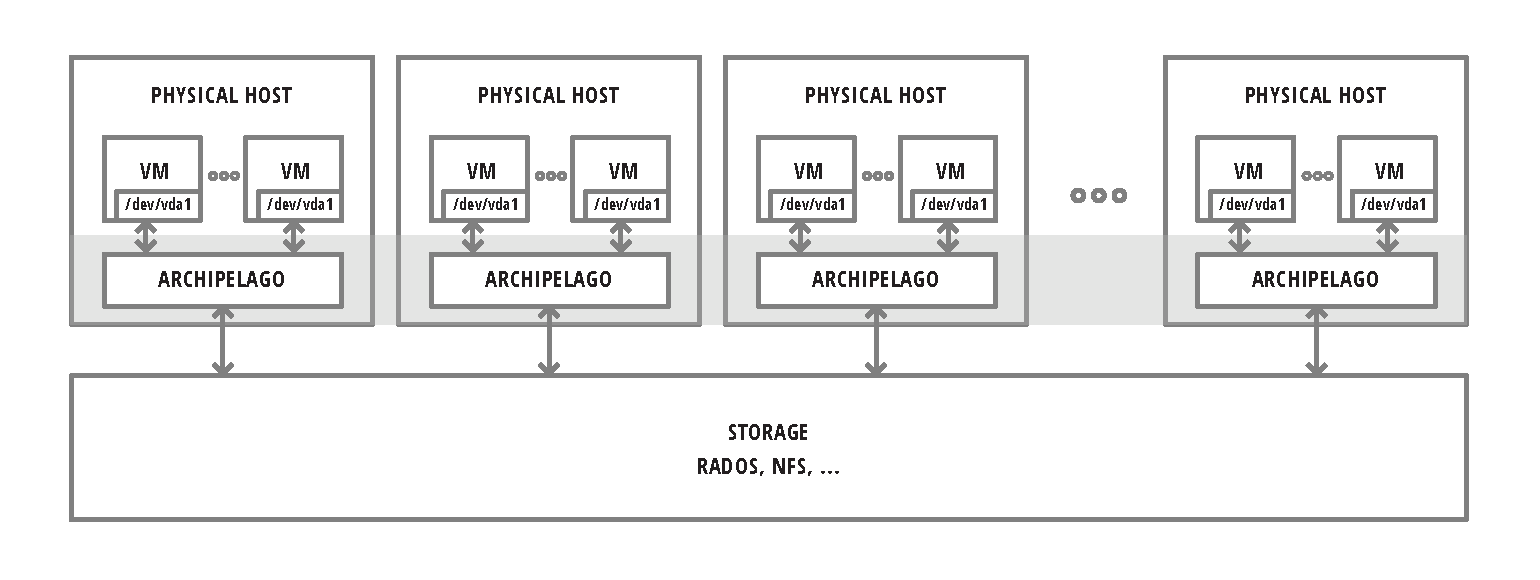
\includegraphics[width=\textwidth]{images/archipelago_overview_a.pdf}}

	\spc

	Key features:
		1) Software-defined
		2) Distributed
		3) Modular
		4) Copy-On-Write
		5) Storage agnostic

	\note{Η λύση που χρησιμοποιήσαμε είναι το Archipelago}
	\note{
		\begin{itemize}
			\item Software-defined: αν και είναι ένα όρος 
				μαρκετινγκ, εμείς κανονικά. Σημαίνει με το 
				software ΟΡΙΖΕΙΣ το storage (εφαρμογή policy, 
				αλλαγή πορείας του request)
			\item τρέχει σε πολλούς κόμβους
			\item αποτελείται από διακριτά κομμάτια
			\item κάνει CoW (εξήγησε ότι τα images είναι λίγα, τα
				VMs πολλά, όπως όταν ένα process κάνει fork)
			\item μπορούμε χρησιμοποιήσουμε ότι storage θέλουμε
		\end{itemize}
	}

\end{frame}

\begin{frame}{Archipelago Architecture}
	%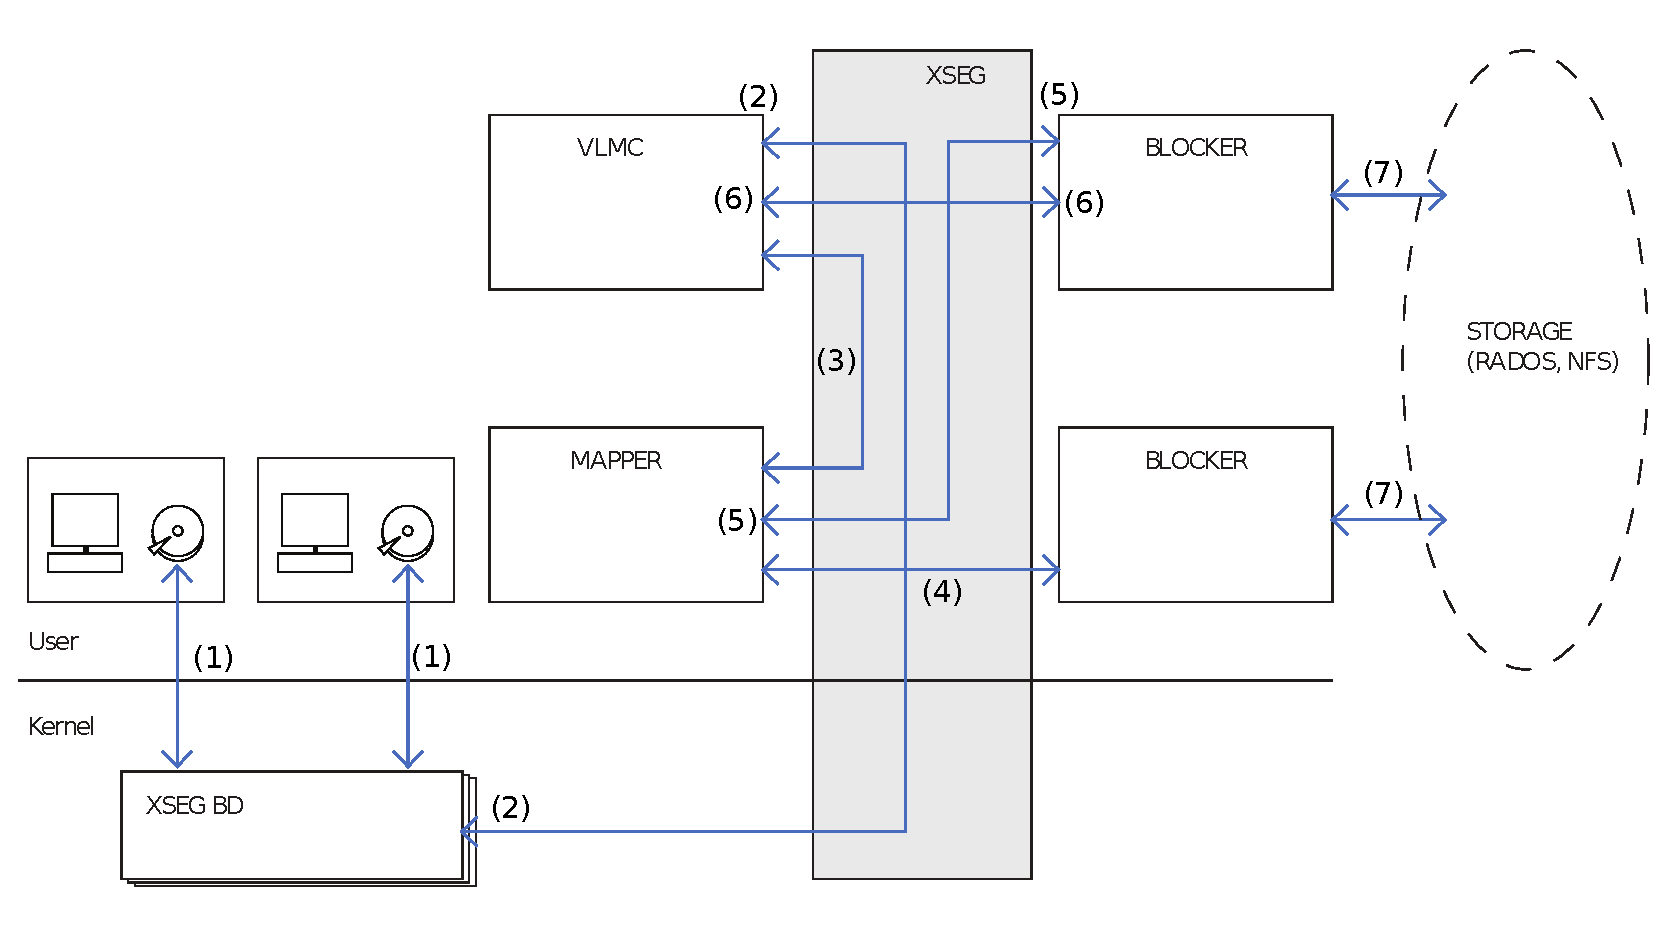
\includegraphics[{images/new_sxima_numbered.pdf}
	\begin{center}
		  \makebox[\textwidth]{\includegraphics[width=0.9\paperwidth]{images/new_sxima_numbered.pdf}}
	\end{center}

	\note[item]{To VM στέλνει αίτημα στο δίσκο του, ο δίσκος είναι εικονικός, 
		θα το δει ο hypervisor (εξήγησε τι είναι ο hypervisor) και θα το 
		στείλει στον δίσκο που το έχουμε πει. (xsegbd)}
	\note[item]{Ο xsegbd στέλνει τo αίτημα στο userspace κομμάτι του 
		Αρχιπελάγους το οποίο αποφαίνεται για τα αντικείμενα τα οποία 
		αντιστοιχούν στο αίτημα. Συνοπτικά πως γίνεται αυτό:
		\begin{itemize}
			\item Ο xsegbd στέλνει το αίτημα στο vmlmc
			\item Ο vlmc συμβουλεύεται τα mappings του
		\end{itemize}
	}
	\note[item]{μετά τα ζητάει από το storage μέσω των blockers}
\end{frame}

\begin{frame}{RADOS}

	The object store component of Ceph filesystem.\\
	\spc
	Key features:
	\begin{itemize}
		\item Replication
		\item Fault tolerance
		\item Self-management
		\item Scalability
	\end{itemize}

	\note{Αν και είμαστε storage agnostic, χρησιμοποιούμε ένα σημαντικό 
		storage backend, το RADOS, που μας δίνει τα εξής:
		\begin{itemize}
			\item Αντίγραφα ασφαλείας των δεδομένων
			\item Ανοχή στο χάσιμο αποθηκευτικών κόμβων
			\item Load balancing και αυτοδιαχείριση
			\item και τέλος ειναι επεκτάσιμο
		\end{itemize}
		\spc\click
	}

	\pause

	\spc
	Speed issues:\\
	VM with page-cache: > 90MB/s, < 1ms\\
	VM without page-cache: < 7MB/s, \mytilde10ms

	\note{Αυτό το περίπλοκο σύστημα όμως δεν είναι αρκετά ταχύ.  
		Παράδειγμα...
		\spc\click}
	\pause

	\spc
	Thesis goal: make this faster.

\end{frame}

